\chapter{Test of Vanna-Volga Pricing}


\section{Data Source}
\subsection{Volatility Matrix}
\paragraph{}
Volatity matrix data in terms of ATM, $10\Delta$, and 25$\Delta$ butterflies (BF) and risk reversals (RR) with three FX derivatives for Vanna-Volga models was sourced from Bloomberg. An example of volatility matrix data of EUR/USD observed on May 10, 2017 with 1M maturity was showing below. More volatility matrix data of other derivatives had been put in \textit{Appendix 1}.

\begin{figure}[htb]
	\centering
	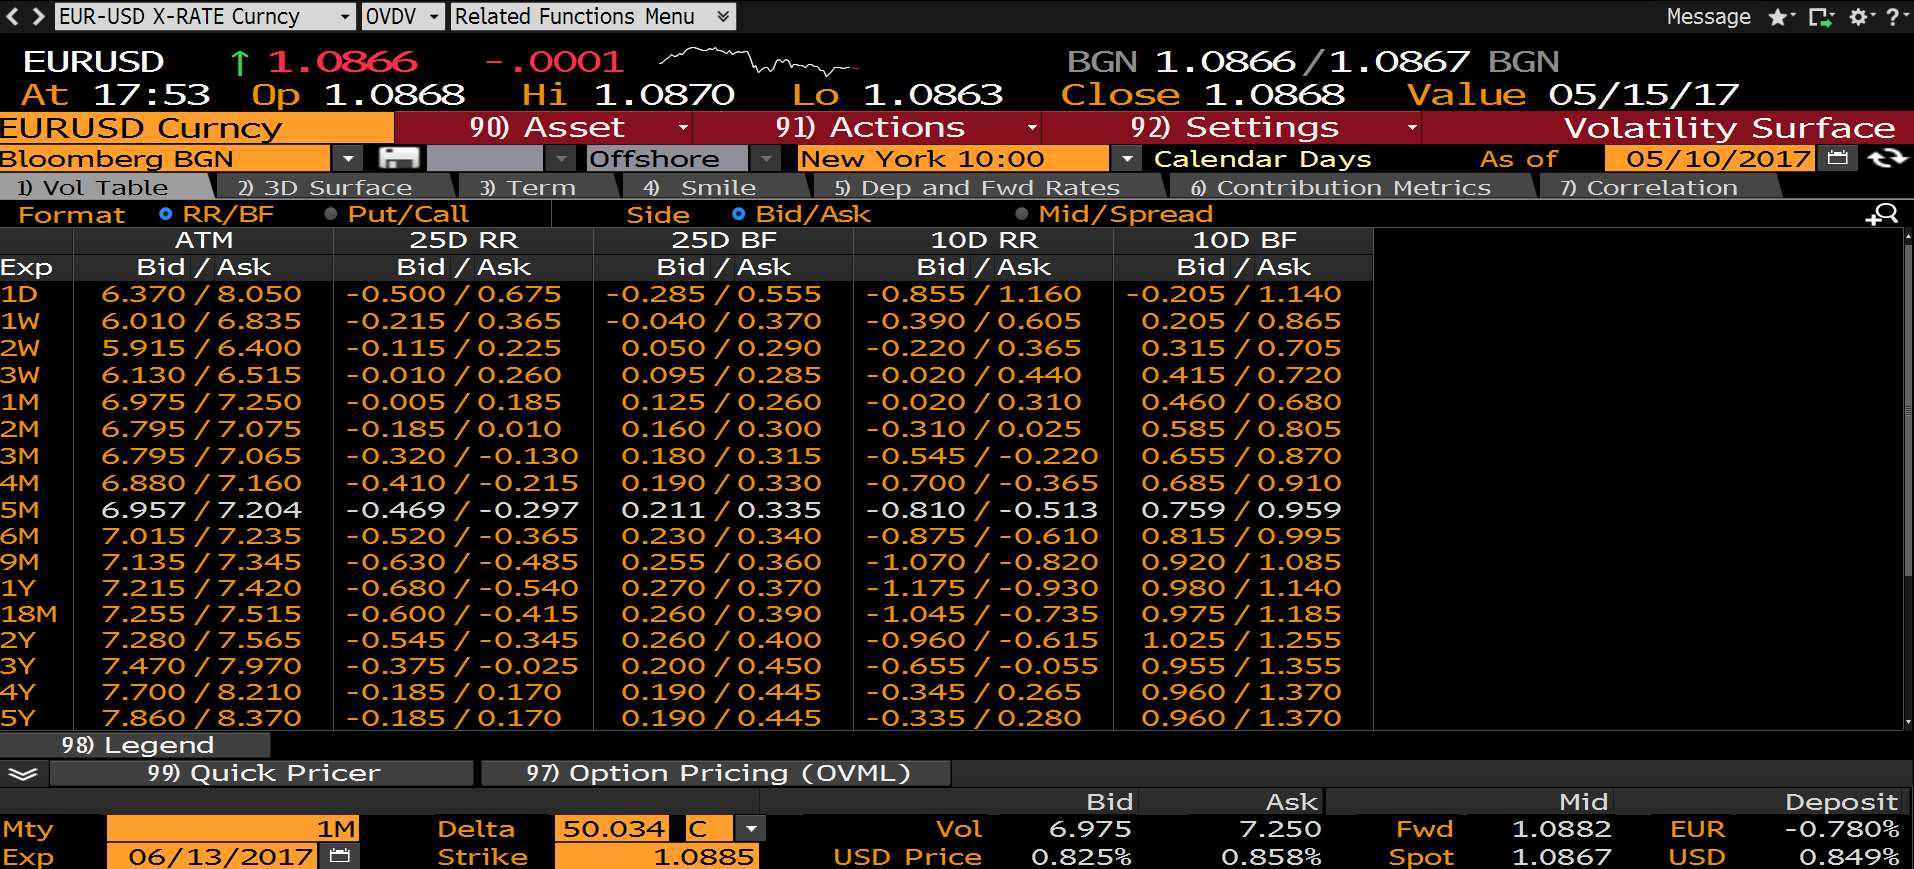
\includegraphics[scale=0.3]{./Testing-data/EURUSD.png} 
	\caption{Volatility matrix data in the bid/ask format in terms of ATM, $10\Delta$, and $25\Delta$ butterflies (BF) and risk reversals (RR), observed on May 10, 2017. Source: \textit{Bloomberg}}
	\label{fig:label} % insert suitable label, this is used to refer to a fig from within the text as shown above
\end{figure}

\paragraph{}
In order to verify the price calculated by using Vanna-Volga model, two benchmark sources (Bloomberg pricing model and \textit{investing.com} with price provided by \textit{Sentry Derivatives}) for all three FX derivatives had been put in \textit{Appendix 1}. Since Vanna-Volga is an analytically derived correction to Black-Scholes model, the price calucluated by Black-Scholes model also had been included for analysis.

\paragraph{}
The interest rates used for Vanna-Volga model and Black-Scholes model was obtained from \textit{www.tradingeconomics.com} and listed in the following table.

\begin{table}[htb]
\centering
\caption{{FX interest rates observed on May 10, 2017}}
\begin{tabular}{ccccc}
\hline	\hline % insert double horizontal line
Symbol & USD & EUR & GBP & JPY \\ [1ex]% heading
\hline
Rates & 1.00\% & 0.00\% & 0.00\% & -0.10\%  \\ [1ex]
\hline
\end{tabular}
\label{table:FX_rates}
\end{table}

\subsection{Model Implementation}
\paragraph{}
As the volatility matrix obtianed from Bloomberg is in the bid/ask format, the averaged mid volatility was used for Black-Scholes model and Vanna-Volga model. The mid volatility matrix data of three FX derivatives were list below. And we consider that live exchange rate as the initial price of FX options $S_0$.

\begin{table}[htb]
\centering
\caption{Mid volatiloty matrix}
\begin{tabular}{ccccccc}
\hline \hline
FX derivatives & ATM  & 25D RR  & 25D BF  & 10D RR  & 10D BF & $S_0$\\ [0.5ex]
\hline 
EUR/USD  & 7.1125 &0.09& 0.1925 &0.145 &0.57&1.0866 \\
GBP/USD & 6.7125 &-0.28&0.2275&-0.4825&0.635&1.2933\\
USD/JPY & 8.225 & -0.4125 &0.2225&-0.775&0.615&114.32\\[0.5ex]
\hline
\end{tabular}
\end{table}

\paragraph{}
With the conventions and definitions specified in \textbf{Technical Specification}, the implementation of Black-Scholes model and Vanna-Volga model of FX derivatives had been coded in jupyter notebook with Python 3.5 in \textit{Appendix 2}.

\section{Testing Results}
\paragraph{}
USD/GBP, USD/JYP, USD/EUR, historical interest rate, historical exchange rate, bloomberg 25delta
Bloomberg: OVDL EUR/USD

price form: \%EUR is price calculated (EUR Pips in \textit{intesting.com}) devide by $S_0$: the exchange rate, i.e., $\%EUR=\frac{EUR Pips}{S_0}$


